\documentclass{article}
\usepackage{ctex}
\usepackage[a4paper,left=10mm,right=10mm,top=15mm,bottom=15mm]{geometry}
\usepackage{graphicx}
\usepackage{amsfonts,amssymb}
\usepackage{amsmath}
\usepackage{biblatex}
\usepackage{hyperref}
\usepackage{color}
\usepackage{titlesec}
\usepackage{titletoc}

\title{代码大全笔记}
\author{张谦}
\date{\today}
\begin{document}
\maketitle
\tableofcontents
\newpage

\section{欢迎进入软件构件的世界}
\subsection{什么是软件构建}
如下图所示,构建活动主要是编码与调试,但也涉及详细设计、规划构建、单元测试、集成、集成测试
等其他活动。
\begin{figure}[ht]
    \centering
    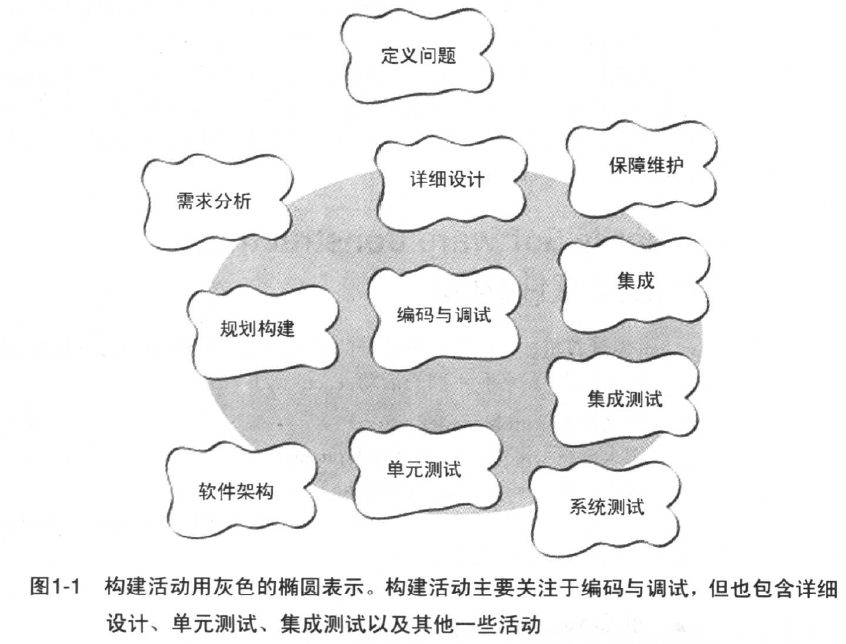
\includegraphics[width=10cm]{figure1.png}
\end{figure}

\par
构建活动包含如下具体任务:
\begin{itemize}
    \item 验证有关的基础工作已经完成,保证构建活动可以顺利进行;
    \item 确定如何测试所写的代码;
    \item 设计并编写类和子程序;
    \item 创建并命名变量和具名常量;
    \item 选择控制结构,组织语句块;
    \item 对代码进行单元测试和集成测试,并排除其中的错误;
    \item 评审开发团队其他成员的底层设计和代码,并让他们评审你的工作;
    \item 优化代码,仔细进行代码的格式化和注释;
    \item 将单独开发的多个组件集成为一体;
    \item 调整代码,让它更快、更省资源。
\end{itemize}

\subsection{构建为什么重要}
\begin{itemize}
    \item 构建活动是软件开发的主要组成部分;
    \item 构建活动是软件开发中的核心活动;
    \item 将主要精力集中于构建活动,可以大大提高程序员生产率;
    \item 构建活动的产物,源代码,往往是对软件的唯一精确描述;
    \item 构建活动是唯一一项确保完成的工作。
\end{itemize}

\section{用隐喻理解软件开发}
隐喻是启示而不是算法,可以将软件开发过程与其他熟悉的活动联系在一起,帮助更好地理解开发过程。
相比其他隐喻,例如写作、种植和养殖等,通过将软件的构建过程,比作房屋的建设过程,能够更好地
理解软件构建的各个阶段。
\subsection{建造隐喻}
\par
(1)问题定义(problem definition):决定准备建一个什么类型的房子;
\par
(2)架构设计(architectural design):和某个建筑师探讨总体设计,并得到批准;
\par
(3)详细设计:画出详细的蓝图,雇一个承包人;
\par
(4)软件构建(construction):准备好建造地点,打好地基,搭建房屋框架,砌好边墙,盖好房顶,
通好水、电、煤气等;
\par
(5)软件优化:在房子大部分完成后,庭院设计师、油漆匠和装修工还要把新盖的房子以及里面的家什
美化一番;
\par
(6)评审和审查(reviews,inspections):在整个过程中,还会有各种监察人员来检查工地、地基、
框架、布线以及其他需要检查的地方。

\subsection{已有组件}
当开发软件时,会大量使用高级语言所提供的功能,而不会自己去编写操作系统层次的代码;
自己编写那些能买得到的现成程序库是没有意义的,例如一些容器类、科学计算函数、用户界面组件、
数据库访问组件等。在建造房子的时候,你也不会去试着建造那些能买得到的东西,例如洗衣机、
冰箱、餐桌等。

\subsection{订制组件}
如果想建造一间拥有一流家具的高档住宅,可能就需要订制的橱柜,以及和橱柜搭配的洗碗机和冰箱等。
在软件开发中也有这种订制的情况,例如想要开发一款一流的软件产品,可能会自己编写科学计算函数,
以便获得更快的速度和更高的精度。

\subsection{防止过度计划}
适当的多层次规划对于建造房屋和构建软件都是有好处的,如果按错误的顺序构建软件,那么编码、测试和
调试都会很难。精心计划,并不是事无巨细的计划或过度计划,例如你可以把房屋的结构性支撑规划清楚,
在日后再决定是用木地板还是瓷砖地板,墙面漆成什么颜色等。

\subsection{不同软件项目}
建筑业中,盖一间仓库或工具房,或是一座医院或核反应站,在规划、设计和质量保证方面所需达到的程度
是不一样的,所用的方法也不相同。同理,在软件开发中,通常只需要用灵活的、轻量级的方法,但有时
你就必须用严格的、重量级的开发方法,以达到所需的安全性目标或其他目标。
另外,还需要特别关注工作时间,在建造帝国大厦时,每辆运料车运输时都留有15分钟的余地,如果
某辆车没能在指定的时间到位,则整个工期就会延误。对于超大型的软件项目,就需要比一般规模的项目
有更高级的规划设计,如果需要创造在经济规模上可以匹敌帝国大厦的庞大软件项目,那么与之相当
水准的技术与管理控制也是必需的。

\section{构建前期准备}
\subsection{前期准备的重要性}
准备工作的中心目标就是降低风险,软件开发中最常见的项目风险是糟糕的需求分析和糟糕的项目计划,
因此准备工作就倾向于集中改进需求分析和项目规划。
高质量的实践方法在项目的初期、中期和末期都强调质量:
\par
(1)如果在项目末期强调质量,那么你会强调系统测试;但是测试只是完整的质量保证策略的一部分,
而且不是最有影响的部分;
\par
(2)如果在项目中期强调质量,那么你会强调构建实践;
\par
(3)如果在项目开始阶段强调质量,那么你就会计划、要求并设计一个高质量的产品;例如你用为吉利车
做的设计来开始整个生产过程,尽管你可以想尽办法来测试,它也绝对不会变成奔驰;也许你能造出最好
的吉利车,但是如果你想要的是奔驰,那么你就得从头开始做设计。

\subsection{序列式开发和迭代式开发选择}
绝大多数的项目都不会完全使用序列式开发法或完全使用迭代式开发法。预先详细说明100\%的需求
和设计是不切实际的,不过对绝大多数项目来说,尽早把那些最关键的需求要素和架构要素确定下来,
时很有价值。
\par
可能因为下列原因选择一个更加迭代的方法:
\begin{itemize}
    \item 需求并没有被理解透彻,或者出于其他理由你认为它是不稳定的;
    \item 设计很复杂,或者有挑战性,或者两者兼具;
    \item 开发团队对于这一应用领域不熟悉;
    \item 项目包含许多风险;
    \item “长期可预测性”不重要;
    \item 后期改变需求、设计和编码的代价很可能比较低。
\end{itemize}
相反的,你可能需要选择一个更加序列的方法。

\subsection{问题定义的先决条件}
在开始构建之前,首先要满足的一项先决条件是,对这个系统要解决的问题做出清楚的陈述。
问题定义只定义了问题是什么,而不涉及任何可能的解决方案。它是一个很简单的陈述,并且听起来
应该像个问题。例如“我们跟不上客户的订单了”听起来就像个问题,而且确实是一个很好的问题
定义;而“我们需要优化数据自动采集系统,使之跟上客户的订单”,这种就是糟糕的问题定义,
它听起来不像问题,而像解决方案。另外,问题定义应该用客户的语言来书写,而且应该从客户的
角度来描述问题。

\subsection{需求的先决条件}
“需求”详细描述软件系统应该做什么,这是达成解决方案的第一步。需求明确有如下好处:
\begin{itemize}
    \item 用户可以自行评审,并进行核准;否则程序员就常常会在编程期间自行决定需求;
    \item 有助于避免争论,如果你和另外一个程序员有分歧,可以查看书面的需求,已解决分歧;
    \item 有助于减少开始编程开发之后的系统变更的情况;
    \item 充分详尽地描述需求,是项目成功的关键,它甚至很可能比有效的构建技术更重要。
\end{itemize}

\par
在构建期间处理需求变更,有以下一些可以采用的方式:
\begin{itemize}
    \item 评估需求质量,如果需求不够好,则停止工作,退回去,先做好后再继续前进;
    \item 确保每一个人都知道需求变更的代价;
    \item 建立一套变更控制程序;
    \item 使用能适应变更的开发方法;
    \item 放弃这个项目;
    \item 注意项目的商业案例,注重商业价值。
\end{itemize}

\subsection{架构的先决条件}
软件架构是软件设计的高层部分,是用于支持更细节设计的框架。架构的质量决定了系统的“概念完整性”,
继而决定了系统的最终质量。一个经过慎重考虑的架构,为“从顶层到底层维护系统的概念完整性”,提供
了必备的结构和体系,它为程序员提供了指引,其细节程度与程序员的技能和手边的工作相配;它将
工作分为几个部分,使多个开发者或多个开发团队可以独立工作。
\par
架构的典型组成部分:
\par
(1)程序组织:
\begin{itemize}
    \item 系统架构首先要以概括的形式对有关系统做一个综述;
    \item 在架构中,应该能发现对那些曾经考虑过的,最终组织结构的,替代方案的记叙;
    找到之所以选用最终的组织结构,而不是其他替代方案的理由;
    \item 架构应该定义程序的主要构造块,根据程序规模的不同,各个构造块可能是单个类,也可能是由
    许多类组成的一个子系统;
    \item 应该明确定义各个构造块的责任,每个构造块应该负责某一个区域的事情,并且对其他构造块负责的
区域知道得越少越好,将设计的信息局限在各个构造块之内;
    \item 应该明确定义每个构造块的通信规则,对于每个构造块,架构应该描述它能直接使用那些构造块,能
间接使用哪些构造块,不能使用哪些构造块。
\end{itemize}

\par
(2)主要的类:
\begin{itemize}
    \item 架构应该详细定义所用的主要的类,应该指出每个主要的类的责任,以及该类如何与其他类交互;
    它应该包含对类的继承体系、状态转换、对象持久化等的描述;如果系统足够大,它应该描述如何将
    这类组织成一个个子系统;
    \item 架构应该记述曾经考虑过的其他类设计方案,并给出选用当前方案的理由;架构无需详细说明
    系统中的每一个类,利用80/20法则:对那些构成系统80\%的行为的20\%的类进行详细说明。
\end{itemize}

\par
(3)数据设计:
\begin{itemize}
    \item 架构应该描述所用到的主要文件和数据表的设计。它应该描述曾经考虑过的其他方案,并说明
    选择当前方案的原因。如果应用程序要维护一个客户ID的列表,而架构师决定使用顺序访问的列表来
    表示该ID的列表,那么文档就应该解释为什么顺序访问的列表比随机访问的列表、堆栈、散列表要好。
    在构建期间,这些信息让你能洞察架构师的思想;在维护阶段,这种洞察力是无价之宝。离开它,你就像
    看一部没有字幕的外语片;
    \item 数据通常只应该由一个子系统或一个类直接访问;例外的情况就是通过访问器类或访问器子程序,
    以受控且抽象的方式来访问数据;
    \item 架构应该详细定义所用数据库的高层组织结构和内容;架构应该解释为什么单个数据库比多个数据库
    要好,反之亦然。需要解释为什么不用平坦的文件,而要用数据库,指出与其他访问同一数据的程序的
    可能交互方式,说明创建哪些数据视图等等。
\end{itemize}

\par
(4)业务规则:
\par
如果架构依赖于特定的业务规则,那么它就应该详细描述这些规则,并描述这些规则对系统设计的影响。例如,
假定要求系统遵循这样一条业务规则:客户信息过时的时间不能超过30秒。在此种情况下,架构就应该描述
这条规则对架构采用的“保持客户信息及时更新且同步”的方法的影响。

\par
(5)用户界面设计:
\par
\begin{itemize}
    \item 用户界面常常在需求阶段进行详细说明,如果没有,就应该在软件架构中进行详细说明。架构
    应该详细定义Web页面格式、GUI、命令行接口等主要元素;
    \item 架构应该模块化,以便在替换为新用户界面时,不影响业务规则和程序的输出部分。例如,架构应该
    使我们很容易做到:砍掉交互式界面的类,插入一组命令行的类。这种替换能力常常很有用,由其
    因为命令行界面便于单元级别和子系统级别的软件测试。1
\end{itemize}

(6)资源管理:
\par
架构应该描述一份管理稀缺资源的计划。稀缺资源包括数据连接、线程、句柄等。在内存受限的应用领域,如
驱动程序开发和嵌入式系统中,内存管理是架构应该认真对待的另一个重要领域。架构应该应该估算在正常情况和
极端情况下的资源使用量。在简单的情况下,估算数据应该说明:预期的运行环境有能力提供所需的资源,
在更复杂的情况下,也许会要求应用程序更主动地管理其拥有的资源。如果是这样,那么资源管理器应该和
系统的其他部分一样,进行认真的架构设计。

\par
(7)安全性:
\par
架构应该描述实现设计

\section{关键的构建决策}


\section{软件构件中的设计}

\section{可以工作的类}

\section{高质量的子程序}

\section{防御式编程}

\section{伪代码编程过程}

\section{使用变量的一般事项}

\section{变量名的力量}


\section{基本数据类型}

\section{不常见的数据类型}

\section{组织直线型代码}

\section{条件语句}

\section{控制循环}

\section{不常见的控制结构}

\section{表驱动法}

\section{一般控制问题}

\section{软件质量概述}

\section{协同构建}

\section{开发者测试}

\section{调试}

\section{重构}

\section{代码调整策略}

\section{代码调整技术}

\section{程序规模对构建的影响}

\section{管理构建}

\section{集成}

\section{编程工具}

\section{布局与风格}

\section{自说明代码}

\section{个人性格}

\section{软件工艺}

\section{更多信息}
顶顶顶

\begin{thebibliography}{99}  
    \bibitem{Meyer2000}Meyer CD (2000) Matrix Analysis and Applied Linear Algebra. Philadelphia, PA: SIAM.
    \bibitem{consistency} Agostino Martinelli. Closed-form solution of visual-inertial structure from motion. International
    Journal of Computer Vision, Springer Verlag, 2013. ￿hal-00905881
\end{thebibliography}



\end{document}

